\chapter{Développement du système}
\lhead{Chapitre 4 - Développement du système}
\section{Introduction}
Le but poursuivit par ce chapitre est d'expliquer les choix qui ont influencé le développement de l'application et de chacun de ses modules externes (ConstriantChecker, XlsParser et GraphParser).

La structure du chapitre sera la suivante. 

La première section présentera l'architecture de l'application et de ses différents modules. On évitera ici de parler de l'architecture MVC car très peu de choix ont été faits à ce niveau  (peu de libertés sont laissées par le framework au final). L'application gère et échange (avec ses modules) une grande quantité de données. Leur modélisation a un impact critique sur les fonctionnalités de l'application (et leur implémentation). C'est pourquoi, l'accent sera mis ici sur la modélisation des classes de l'application.   

La deuxième section présentera les choix faits au niveau de l'implémentation des différentes fonctionnalités. Il sera expliqué par la même occasion comment ces fonctionnalités ont été implémentées. 


\label{developpement_system}

\section{Architecture}

\subsection{Architecture globale}

\begin{figure}
\caption{Architecture globale}
\centering
\label{fig:complete_arch}
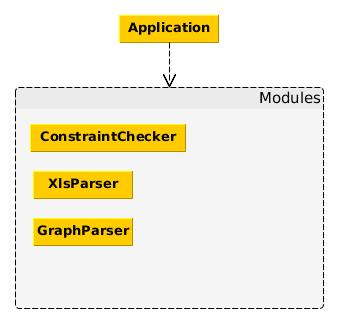
\includegraphics[scale = 0.5]{complete_arch}
\end{figure}

Ce modèle représente l'architecture de l'application et de l'ensemble de ses modules. L'objet application représente la partie \textit{Rails} de l'application. Cette partie comporte essentiellement les différents modèles, leurs vues et leurs contrôleurs (en plus de la base de données). L'application utilise trois modules développés indépendamment.
\begin{enumerate}
  \item \textbf{GraphParser} - le module s'occupant d'extraire l'information contenue dans les fichiers \textit{Graphml} générés par yEd, 
  \item \textbf{ConstraintCheker} - le module s'occupant de vérifier les contraintes des programmes d'étudiants
  \item \textbf{XlsParser} - le module occupant d'exporter les données relatives aux programmes de cours vers un formulaire Excel et d'extraire les informations contenues dans les formulaires Excel que la commission importe via l'application. 
\end{enumerate}

Les informations manipulées par ces trois modules sont présentées en détail dans la section relative à la gestion des données du chapitre précédent \ref{data_mgmt}.

L'architecture de chacun de ces modules, en plus de celle de l'application, sera expliquée dans les sous-sections qui suivent. Notez que la notation UML sera utilisée pour présenter les différents diagrammes de classe. 


%*********************$$
\clearpage
\subsection{Application Rails}
\label{rails_arch}

Il y a plusieurs types d'associations en Ruby on Rails;
\begin{itemize}
  \item l'association de cardinalité  (0..1, 1..1) est représentée par la double relation A has one B et B belongs to A; l'id de l'objet A étant stocké dans la table de l'objet B;
  \item l'association de cardinalité (0..*, 1..*) est représentée par la double relation A has many B et B belongs to A; l'id de l'objet A étant stocké dans chacun des objets B qui est en relation avec A;
  \item l'association de cardinalité (0..*, 0..*) est représentée par la double relation has and belongs to many entre A et B; les ids de chacun des objets sont stockés dans une table intermédiaire. 
\end{itemize}

\label{arch}
\begin{figure}
\centering
\caption{Architecture de l'application}
\label{fig:app_arch}
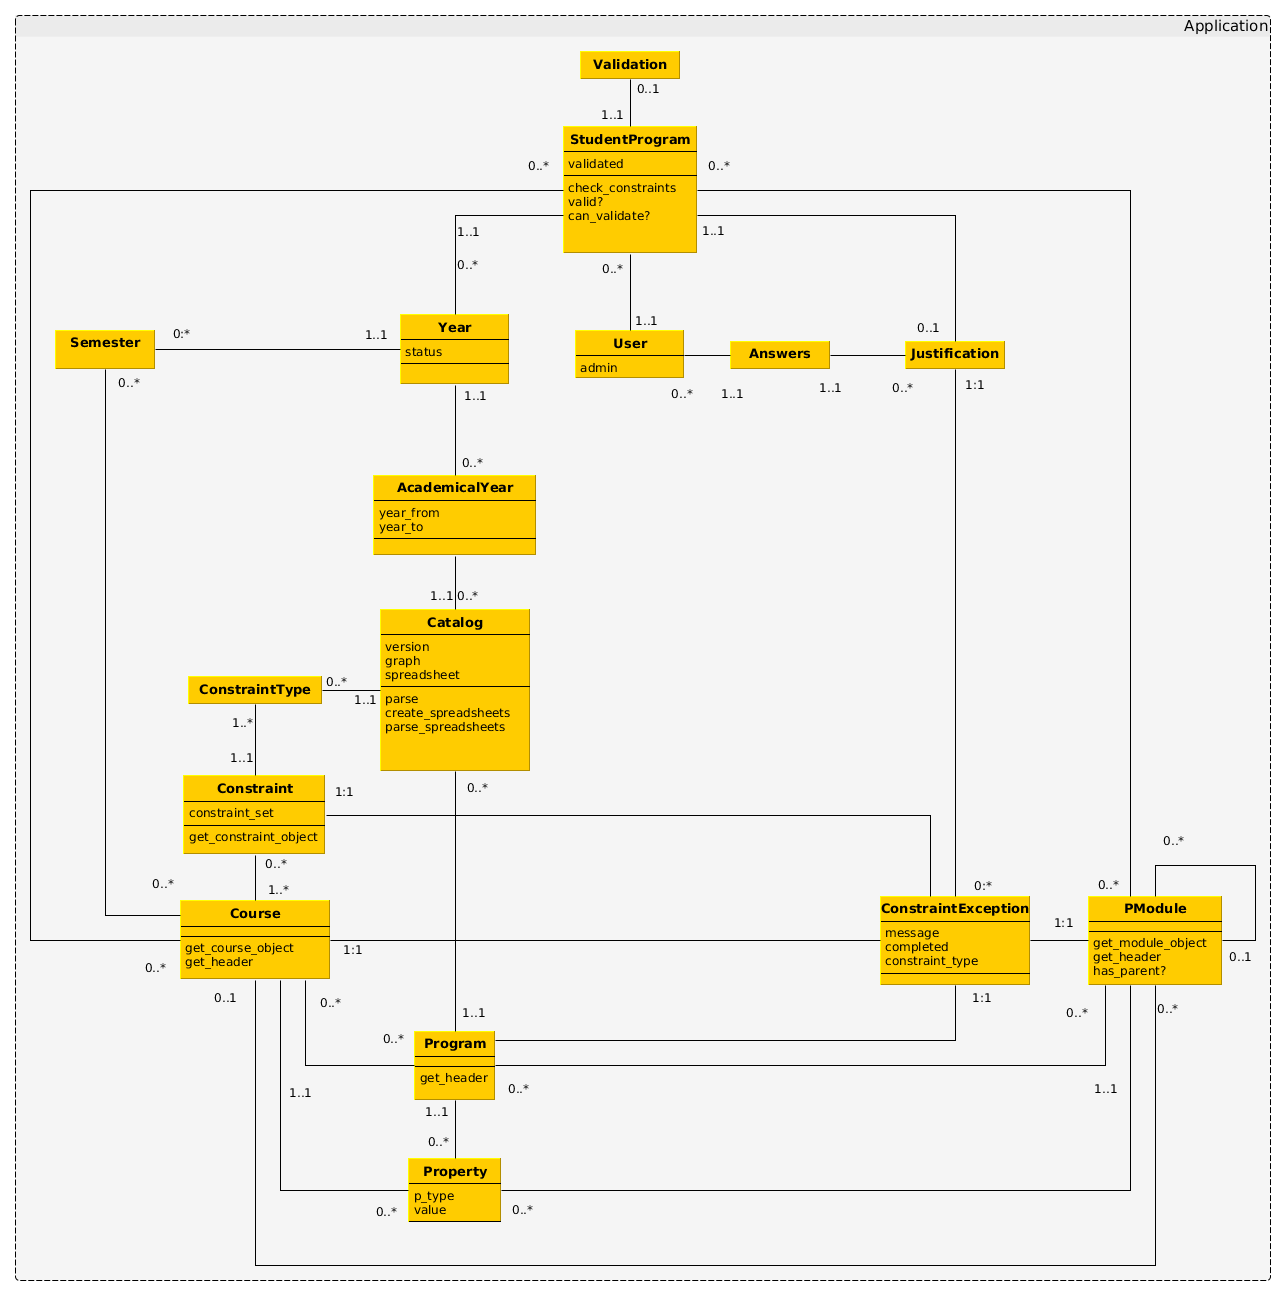
\includegraphics[width=\textwidth]{app_arch}
\end{figure}

\subsubsection{User} 

Cette classe représente les utilisateurs.  L'attribut \textbf{admin} sert à différencier les deux acteurs de l'application, à savoir la \textit{Commission de programme} et les étudiants. La section \ref{user_mgmt}
 explique en détail comment sont gérés les accès de ces deux types d'utilisateurs.

\subsubsection{Property}

Un objet \textit{Property} est composé d'un type et d'une valeur. Chacun des objets \textit{Program}, \textit{PModule} et \textit{Course} peu en avoir zéro ou plusieurs. Par exemple, pour représenter le sigle d'un cours, une propriété de type \textit{SIGLE} et de valeur \textit{SINF1101} sera ajoutée au cours correspondant. Il a été choisi d'opter pour cette solution, plutôt que d'ajouter des champs arbitraire (Sigle, crédits, ...) à chacun des objets car on ne sait pas à l'avance quelles seront leur propriété. En effet, elle sont déterminées par les informations mises dans le fichier excel qui est importé régulièrement dans l'application. 

\subsubsection{PModule}

C'est un ensemble de cours. Un \textit{PModule} peut avoir plusieurs \textit{PModule}. Ce comportement est justifié par le fait qu'un module de cours peut comporté un sous module qui comporte une série de cours obligatoires (L'option réseau et l'ensemble de ses cours obligatoires par exemple).

\subsubsection{Program}

Il représente un programme de cours. (Le programme de master par exemple) C'est un ensemble de cours et de modules divers. On peut créer des programmes via l'outil de graphes yEd, mais il est possible dans l'application de créer des Programmes \textit{à la carte} en choisissant les modules et cours qui le compose. C'est pourquoi il y a une relation \textit{many to many} entre \textit{PModule} et \textit{Program} et une autre entre \textit{Program} et \textit{Course}. En effet, chaque Programme peut avoir un ou plusieurs cours, et chaque cours peut appartenir à un ou plusieurs programmes (Le même comportement est observé pour les modules). Il n'est donc pas possible de représenter cette relation avec une relation \textit{has many} classique.

\subsubsection{Catalog}

Un catalogue est la représentation d'un graphe généré avec le logiciel yEd en base de données.Il est composé de plusieurs \textit{Program}, \textit{PModule} et \textit{Course}. Il contient aussi les informations à propos du fichier de graphe et du formulaire excel (nom, date, type). 

L'attribut \textit{version} est un entier qui représente la version du catalogue de cours. Il peut prendre trois valeurs différentes:

\begin{itemize}
  \item version \textit{future}, représentée par l'entier 0;
  \item version \textit{principale}, représentée par l'entier 1;
  \item version \textit{ancienne}, représentée par l'entier 2.
\end{itemize}

La version du catalogue est utilisée pour identifier les catalogues qui sont utilisables par les étudiants (version principale et ancienne) de ceux qui sont encore à l'état de \textit{draft}. Les anciens catalogues contiennent les informations (propriétés et contraintes) liées au années réussies ou ratées. Les contraintes et propriétés évoluant chaque année, il est nécessaire de garder la trace des anciennes pour que les programmes des étudiants restent valides au fur et à mesure que les catalogues évoluent.

Les trois méthodes principales de cette classes sont:

\begin{description}
  \item[import\_graph] qui appelle le module \textit{GraphParser}
  \item[import\_catalog\_data] qui extrait les informations du formulaire excel (et upload la nouvelle version du formulaire sur le cloud).
  \item[export\_catalog\_data] qui crée le formulaire excel (et l'upload sur le cloud).
\end{description}

Les détails d'implémentation de ces méthodes seront expliquées dans la section relative au module avec lequel elles interagissent. 

\subsubsection{StudentProgram}

C'est le programme que se crée l'étudiant lorsqu'il utilise l'application. Un \textit{StudentProgram} est une instanciation d'un des \textit{Program} disponible dans le \textit{Catalog} utilisé (d'où la relation \textit{many to many}). De plus, un étudiant doit choisir les modules qu'il va suivre. Ce comportement est expliqué par la relation \textit{many to many} entre les deux modèles. Pour configurer son programme année par année, l'étudiant va se créer une ou plusieurs années (\textit{Year})

L'attribut \textit{validated} représente le fait qu'un programme d'étudiant aie été validé ou non par la commission.

La méthode \textit{can\_validate?} vérifie que certaines conditions sont remplies pour pouvoir envoyer un programme d'étudiant à la validation (Se référer à la section \ref{validation_request} pour plus de détail sur cette fonctionnalité).

La méthode \textit{check\_constraints} gère l’interaction avec le module \textit{ConstraintsChecker}. 

\subsubsection{Year}

Une année est composé de plusieurs semestres (deux idéalement). L'attribut \textit{status} représente les trois état dans le quel peut se trouver une année (réussie, ratée ou en cours). Un semestre est représenté par l'objet \textit{Semester}.Le choix de chacun des cours du semestre est représenté par une association \textit{has\_and\_belongs\_to\_many} qui existe entre les deux objets.

Les programmes étant validés par année en s'appuyant sur l'ensemble du programme de l'étudiant, ce modèle est d'autant plus important. En effet, en aucun cas, le programme n'est validé dans son ensemble. 

\subsubsection{Header}

Chacun des modèles \textit{Course}, \textit{Pmodule} et \textit{Program} contient une méthode get\_header qui renvoie une suggestion de noms de propriétés utilisées à titre indicatif avec le module \textit{XlsParser} (voir \ref{xls_parser}) pour créer les formulaires Excel. Nous avons le header suivant : \{"SIGLE", "CREDITS", "SEMESTRE", "OBLIGATOIRE"\} pour le modèle \textit{Course} par exemple.

Si à l'avenir, on découvre une autre propriétés qu'il est important d'avoir dans pour un cours, un programme ou un module, une bonne pratique serait d'ajouter le nom de cette propriété dans ce header!

\subsubsection{Méthodes get\_objet}
Ces méthodes s'occupent de créer les objets qui sont utilisé par le module ConstraintsChecker. Pour un objet du modèle Cours par exemple, il va créer un objet de la classe Cours (spécifique au module \textit{ConstraintsChecker} et des objets pour représenter ces différentes contraintes (dépendances, etc). Ces objets (qui sont spécifiques au module) sont ensuite manipulés par module \textit{ConstraintsChecker}.

\subsubsection{Constraints}
Cette classe représente les dépendances entre les cours. Le type de la dépendance est représenté par le modèle \textit{ConstraintType}. L'attribut \textit{set\_type} quant à lui représente le type de l'ensemble des contraintes. Comme expliqué dans la section \ref{contraintes}, une dépendance peut être une relation binaire entre un cours et sa dépendance. Elle peut être aussi une relation n-aire entre plusieurs cours et leurs dépendances.

Il existe deux associations (bien qu'elles ne soient représentées que par une seule, par soucis de clarté, sur le diagramme de classes \ref{fig:app_arch}) qui relient les objets \textit{constraints} aux objets \textit{courses}. Le modèle \textit{Constraint} ne représente que les contraintes de type dépendance, comme expliqué dans la section \ref{contraintes}. Ce type de contrainte ayant un cours source et un cours destination, il est donc nécessaire d'avoir deux relations.  La relation entre la destination et la contrainte est représentée par une association \textit{has\_many} entre le cours et la contrainte. La relation entre la ou les sources et la contrainte, quant à elle, est représentée par une association \textit{has\_and\_belongs\_to\_many}. 

Ce comportement est justifié par le fait que l'on accède aux contraintes depuis le cours \textit{destination}, c'est à dire que l'on va chercher les dépendances d'un cours, et non chercher la relation inverse, à savoir quels sont les cours pour lesquels un cours joue le rôle de dépendance.

\subsubsection{AcademicYear}
Ce modèle représente une année académique, c'est à cheval sur deux années civiles. Elle est utilisée dans deux situations:
\begin{enumerate}
  \item identifier les objets \textit{Year} 
  \item identifier les objets \textit{Catalogue}; en effet, chaque années lorsque l'on modifie les programmes de cours d'un catalogue, il faut importer le nouveau graphe. On peut ainsi identifier l'année académique à la quelle le catalogue est lié et savoir \textbf{où} aller chercher la nouvelle version du programme que l'étudiant suit lorsqu'une nouvelle année académique commence.
  \item gérer, du coté du module \textit{ConstraintsChecker} les prérequis et les corequis d'un cours. En effet, il est nécessaire de savoir quand a été suivi une dépendance pour savoir si la contrainte est valide ou non. 
\end{enumerate}

\subsubsection{ConstraintException}
Lorsque le module \textit{ConstraintsChecker} a terminer la vérification des contraintes du programme d'un étudiant, il renvoie les contraintes qui ne sont pas valides. Lors de la phase de négociation entre la commission de programme et l'étudiant, ce dernier doit justifier chacune des contraintes qui ne sont pas valides dans son programme.

L'utilité de ce modèle est de faire le lien entre la contrainte non vérifiée, le programme de l'étudiant et le message qui justifie cette exception dans son programme. 

Un objet \textit{ConstraintsChecker} peut être en relation avec;

\begin{itemize}
\item un objet Cours, P\_Module ou un Program lorsqu’il concerne une contrainte, portant sur les propriétés, qui n'est pas valide;
\item un objet Constraint lorsqu'il concerne une dépendance (prérequis par exemple) qui n'est pas valide.
\end{itemize}

De plus il contient;
\begin{itemize}
\item un attribut \textit{constraint\_type} pour différencier les types de contraintes (prérequis disjonctif(OR), minimum de crédits requis, etc);
\item un message qui stocke la justification de l'étudiant.
\end{itemize}

Toute ces exceptions sont stockées dans une instance du modèle \textit{Justification} qui va servir de \textit{médium} entre les deux parties durant la phase de négociation.

\subsection{Architecture du vérificateur de contraintes}
\label{constraintchecker}
\begin{figure}[H]
\centering
\caption{Vérificateur de contraintes}
\label{fig:constraint_checker_arch}
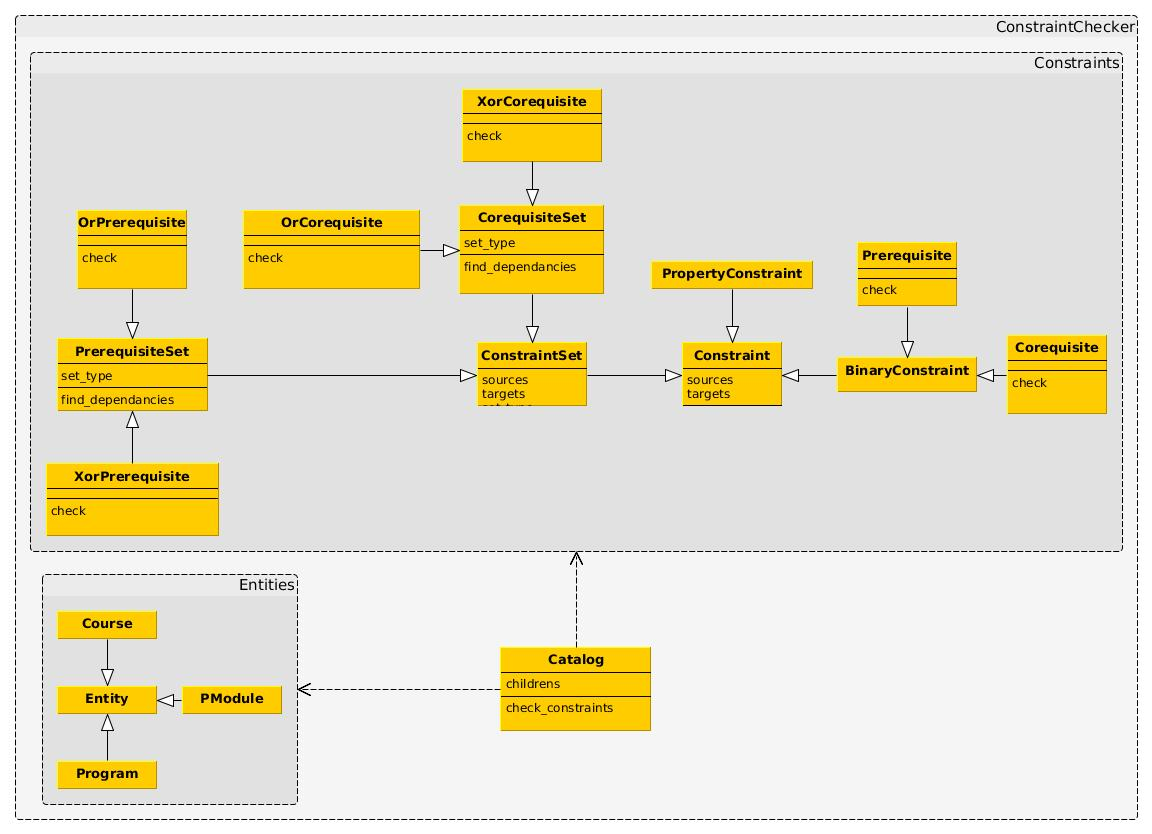
\includegraphics[width=\textwidth]{constraint_checker_arch}
\end{figure}

L'architecture de ce module est composé de deux parties:
\begin{enumerate}
  \item Les différents types de contraintes;
    \begin{itemize}
    \item Corequisite (classe parente : BinaryConstraint);
    \item Prerequisite (classe parente : BinaryConstraint);
    \item OrCorequisite (classe parente : ConstraintSet);
    \item OrPrerequisite (classe parente : ConstraintSet);
    \item XorCorequisite (classe parente : ConstraintSet);
    \item XorPrerequisite (classe parente : ConstraintSet);
    \item Min (classe parente : PropertyConstraint);
    \item Max (classe parente : PropertyConstraint);
    \item Mandatory (classe parente : PropertyConstraint).
    \end{itemize} 
  \item Les différents types d'entités (Cours, modules, programme et student\_program).
\end{enumerate}

Le lien avec l'application se situe au niveau de la classe \textit{StudentProgram}. En effet, chacune des différentes entrées des objets (de la base de données) concernées (courses, p\_modules, constraints) est traduite en un objet entité.

L'idée ici est d'utiliser au plus l'héritage pour éviter d'avoir des duplications de code dans les classes. Par exemple, un objet \textit{Course} peut avoir beaucoup de contraintes mais chacune d’entre elles peut être de n'importe quel type. Cet objet n'a pas besoin de savoir le type de ses contraintes. Tout ce qu'il sait, c'est qu'il doit appeler leur méthode \textit{check} pour tester si les contraintes sont vérifiées. 


\subsection{Parser de graphes}

\begin{figure}[H]
\centering
\caption{Architecture du parser de graphe}
\label{fig:graph_parser_arch}
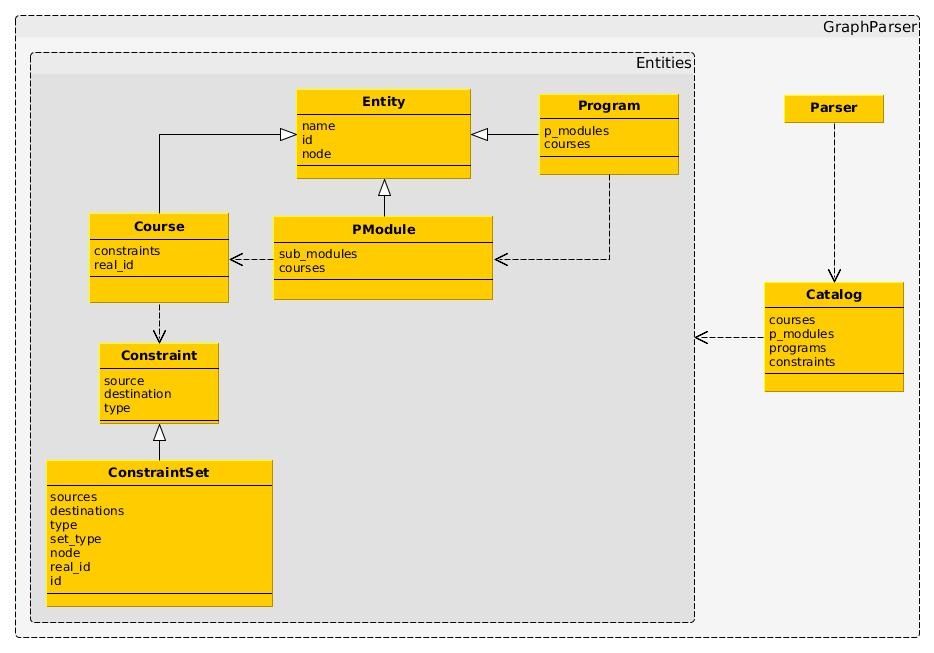
\includegraphics[width=\textwidth]{graph_parser_arch}
\end{figure}



Tout comme dans le vérificateur de contraintes \ref{constraintchecker}, on utilise un objet ruby qui étend la classe \textit{Entity} pour chaque objet de la base de données (courses, p\_module, program). Une fois le graphe parsé, les informations contenues dans ces objets ruby sont ajoutées dans la base de données. 

De nouveau, l'héritage occupe une page prépondérante ici, pour diminuer le couplage, augmenter la cohésion  et éviter autant que possible la duplication de code \cite{cohesion_couplage}. 

\subsection{Parser de fichiers excel}
\label{xls_parser}
\begin{figure}[H]
\centering
\caption{Architecture du parser de fichiers excel}
\label{xls_parser_arch}
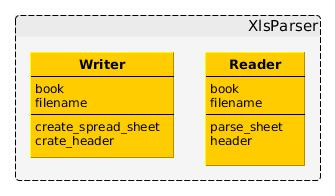
\includegraphics[scale=1]{xls_parser_arch}
\end{figure}

Ce module est relativement simple; il est composé de deux classes, un \textit{Writer} qui prend en input un tableau de données et un \textit{Reader} dont l'output est aussi un tableau de données.


\clearpage
%*************************************************************************************************************************************
\section{Implémentation}
\subsection{Introduction}
Le but de ce chapitre est de présenter les grandes lignes des algorithmes utilisés dans chaque partie de l'application. 
\subsection{Hébergement de l'application}
L'application est hébergée sur \textit{Heroku}. On évite ainsi de devoir s'occuper de la configuration et de la maintenance du serveur qui doit héberger l'application. Cela impose cependant quelques restrictions;
\begin{enumerate}
  \item On est obligé d'utiliser postgresql comme système de base de données.
  \item Le répertoire de l'application est en lecture seule. On ne peut donc pas stocker le fichier de graphe et le formulaire Excel dedans. Il est donc nécessaire d'utiliser un service de \textit{cloud storage} externe à l'application. Amazon S3 à été utilisé pour palier à ce problème. Pour rendre le téléchargement des fichiers vers ce service plus aisé, la gem \textit{Paperclip} a été utilisé. Les détails de configuration de ces différents services sont expliqués en annexes. 
\end{enumerate}
\subsection{Gestion des utilisateurs}
\label{user_mgmt}
Les utilisateurs sont gérés à l'aide de deux gems. 

Devise est utilisé pour tout ce qui concerne la gestion des comptes (Création, modification, suppression), la gestion des sessions (Login/logout) et surtout la création de la table users et des différents attributs requis.

CanCan est utilisé pour tout ce qui concerne les permissions des utilisateurs, à savoir à quels modèles un utilisateur à accès, et quelles actions il peut effectuer sur ces modèles (Read, Create, Destroy, ...) 

Pour gérer les deux types d'utilisateurs (Commission de programme et Étudiants), trois choix s'offrent à nous:
\begin{enumerate}
  \item générer avec Devise deux tables séparées;
  \item utiliser la Single Table Inheritance \cite{STI}. On crée un modèle user, puis on crée deux modèles spécifiques (student et admin) qui héritent de ce premier modèle;
  \item générer un seul modèle user et y ajouter un attribut \textit{admin} pour identifier le rôle de l'utilisateur.
\end{enumerate}

La troisième solution a été choisie. Elle permet d'éviter la redondance induite par la première solution et est plus simple à implémenter et à maintenir que la deuxième solution. En effet nos deux types d'utilisateurs ne diffèrent que par leur rôle. 


% La table générée par devise est la suivante;

% \begin{lstlisting}
%   create_table "users", force: true do |t|
%     t.string   "email",                  default: "",    null: false
%     t.string   "encrypted_password",     default: "",    null: false
%     t.string   "reset_password_token"
%     t.datetime "reset_password_sent_at"
%     t.datetime "remember_created_at"
%     t.integer  "sign_in_count",          default: 0,     null: false
%     t.datetime "current_sign_in_at"
%     t.datetime "last_sign_in_at"
%     t.string   "current_sign_in_ip"
%     t.string   "last_sign_in_ip"
%     t.datetime "created_at"
%     t.datetime "updated_at"
%     t.boolean  "admin",                  default: false
%   end
% \end{lstlisting}

% Pour vérifier si un utilisateur est connecté dans les vues, il suffit d'appeler le helper suivant

% \begin{lstlisting}
% user_signed_in?
% \end{lstlisting}

% Cela nous permet par exemple de cacher à l'utilisateur les menus permettant accéder aux différentes vues s'il n'est pas connecter

% Pour vérifier si l'utilisateur à le rôle admin, il suffit de vérifier l'attribut dans la vue

% \begin{lstlisting}
% current_user.admin?
% \end{lstlisting}

% current\_user représentant l'utilisateur qui est connecté pour le moment.


% Cependant, cela n'est pas suffisant. En effet, cela n'empêche pas l'utilisateur d'accéder aux différentes vues en entrant l'url dans la barre de navigation. C'est pourquoi il est nécessaire de dire à chaque contrôleur qu'il faut vérifier qu'un utilisateur est connecté avant d'afficher les vues. C'est fort heureusement très simple à faire avec Devise. Il suffit d'ajouter la ligne 
% \begin{lstlisting}
% before_action :authenticate_user!
% \end{lstlisting}

% dans chaque contrôleur où il est nécessaire que l'utilisateur soit connecté pour accéder aux vues. 

% \textit{CanCan} intervient pour gérer les accès autorisés aux deux rôles de notre application (Utilisateur normal et admin). Il suffit simplement de créer un modèle \textit{Ability} dans lequel on décrit ce à quoi chaque rôle à accès. C'est de nouveau très simple;

% \begin{lstlisting}
%     if user.admin?
%         can :manage, :all
%     else
%         can :manage, [StudentProgram, Year, Semester]
%         can :create, Validation
%     end
% \end{lstlisting}

% Il suffit de définir, en fonction du rôle de l'utilisateur, les modèles auxquels il a accès et ce qu'il peut faire. L'utilisateur \textit{normal} par exemple, n'a accès qu'aux modèles \textit{StudentProgram, Year, Semester}. S'il tente d'accéder aux vues des modèles auxquels il n'a pas accès, il sera redirigé vers la page d’accueil. 

% Notez qu'il est possible de générer les vues qui permettent à l'utilisateur de s'enregistrer, de se connecter et de gérer les informations relatives à son compte utilisateur. Ces vues ont cependant été modifiées pour que leur style s'adapte à celui de l'application. 

% Enfin, il n'est pas possible, pour des questions de sécurité évidentes, de se créer un compte \textit{admin} via les formulaires d'enregistrement disponibles dans l'application. Il faut tout d'abord se créer un compte utilisateur dans l'application, et ensuite modifier l'attribut \textit{admin} directement dans la console.  

\subsection{Importation du graphe}
\subsubsection{Introduction}
\label{graph_format_justification}
Une fois le graphe créé à l'aide de yEd, plusieurs choix s'offrent à nous pour exporter nos données. Les formats (non binaires) dans lesquels nous pouvons exporter les informations contenues dans notre graphe sont les suivants:
\begin{enumerate}
\item GraphML, un format de fichier basé sur XML pour les graphes;
\item XGML, une alternative au format GraphML, mise en place par yWorks, la société qui développe le logiciel yEd;
\item TGF (Trivial Graph Format) un format de fichier texte relativement simple pour décrire des graphiques.
\end{enumerate}

TGF est de la forme

\begin{lstlisting}
1 SINF1101
2 FSAB1401
3 SINF1103
4 SINF1102
5 SINF1140
6 INGI1123
7 INGI1101
8 FSAB1402
9 NS //(Option network & security du programme Master)
\end{lstlisting}

et contient trop peu d'informations sur le graphe, comme les appartenances des cours aux différents modules et programmes. C'est pourquoi une solution basée sur XML a été choisie.

Un fichier GraphML contient les informations suivantes pour un noeud de type COURS.

\begin{lstlisting}
 <node id="n1::n3" yfiles.foldertype="group">
  <data key="d5"/>
    <data key="d6">
    (...)
  <node id="n1::n3::n2">
      <data key="d5"/>
      <data key="d6">
        <y:ShapeNode>
          <y:Geometry height="30.0" width="68.0" x="1136.0" y="1541.453125"/>
          <y:Fill color="#FFCC00" transparent="false"/>
          <y:BorderStyle color="#000000" type="line" width="1.0"/>
          <y:NodeLabel alignment="center" autoSizePolicy="content" fontFamily="Dialog" fontSize="12" fontStyle="plain" hasBackgroundColor="false" hasLineColor="false" height="17.96875" modelName="internal" modelPosition="c" textColor="#000000" visible="true" width="61.57421875" x="3.212890625" y="6.015625">SINF2335</y:NodeLabel>
          <y:Shape type="rectangle"/>
        </y:ShapeNode>
     </data>
  </node>
  (...)
</node>
\end{lstlisting}

En comparaison, la version \textit{XGML} du même nœud.
\begin{lstlisting}
<section name="node">
  <attribute key="id" type="int">69</attribute>
  <attribute key="label" type="String">SINF2335</attribute>
  <section name="graphics">
    <attribute key="x" type="double">1170.0</attribute>
    <attribute key="y" type="double">1556.453125</attribute>
    <attribute key="w" type="double">68.0</attribute>
    <attribute key="h" type="double">30.0</attribute>
    <attribute key="type" type="String">rectangle</attribute>
    <attribute key="fill" type="String">#FFCC00</attribute>
    <attribute key="outline" type="String">#000000</attribute>
  </section>
  <section name="LabelGraphics">
    <attribute key="text" type="String">SINF2335</attribute>
    <attribute key="fontSize" type="int">12</attribute>
    <attribute key="fontName" type="String">Dialog</attribute>
    <attribute key="anchor" type="String">c</attribute>
  </section>
  <attribute key="gid" type="int">61</attribute>
</section>
\end{lstlisting}

La principale différence entre le format XGML et GraphML se situe au niveau de la structure des informations. XGML structure toute les données de façon linéaire, en ne respectant pas la hiérarchie des différents nœuds et boites.

\begin{figure}
\centering
\caption{Exemple de graphe hiérarchique} 
\label{fig:hierarchical_graph_example}
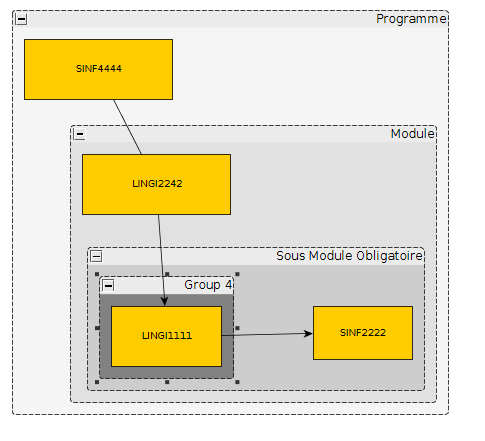
\includegraphics[width=\textwidth]{hierarchical_graph_example}
\end{figure}

Pour le graph \ref{fig:hierarchical_graph_example} par exemple, la structure d'un fichier XGML sera de la sorte:
\begin{lstlisting}
Node Programme
Node SINF4444
Node MODULE
Node LINGI2242
Node SOUS MODULE OBLIGATOIRE
(...)
\end{lstlisting}

Lorsque l'on parsera le fichier, on devra:
\begin{itemize}
  \item Parcourir le fichier, extraire les informations (nom, parent) de chaque cours, module et programme;
  \item Parcourir la liste des cours, modules et programmes pour ajouter les références vers leurs parents et leurs enfants.
\end{itemize} 

Avec GraphML par contre, la structure  du fichier sera la suivante;

\begin{lstlisting}
Node Programme
Childs : [
  Node SINF4444
  Node MODULE
  Childs : [
    Node LINGI2242
    Node SOUS MODULE OBLIGATOIRE
    Childs : [
    ]
  ]
]
(...)
\end{lstlisting}

Lorsqu'on parsera le fichier; on devra simplement extraire les informations comme précédemment. On saura par contre au moment où l'on parse un objet à quel parent il appartient.  Il n'est donc pas nécessaire de retraiter tous les éléments pour compléter les informations à propos de leur parent et de leurs enfants. Ceci est la principale raison pourquoi \textit{Graphml} est le format supporté par l'application.


\subsubsection{Parsing}
\label{graph_parsing}
Le but de ce module est de fournir une abstraction supplémentaire à la gem \textit{Nokogiri}\footnote{Librairie ruby permettant de parser des fichiers XML} pour extraire les informations contenues dans le fichier \textit{GraphML} de yEd. Ce module va, à partir des informations conenues dans le graphe, créer un objet du modèle Catalogue. Les informations contenue dans le graphe généré avec \textit{yEd} sont les suivantes:
\begin{itemize}
\item les Programmes de cours (Bachelier, Masters);
\item les Modules et leur nom;
\item les Sous-modules et leur nom;
\item les cours et leur sigle;
\item les contraintes hiérarchiques (Qui contient quoi);
\item les dépendances entre les cours (Corequis et Prérequis).
\end{itemize}


Ce module est appelé par le modèle \textit{Catalogue} de l'application à sa création. Le fichier graphe est d'abord envoyé sur le  \textit{cloud amazon}, puis parsé par le module \textit{GraphParser}. Une fois le parsing terminé, les différents objets (Cours, Modules et Programmes) sont récupérés par le modèle \textit{Catalogue}, puis traités par chacun des modèles concernés, avant d'être enregistrés en base de données. 

Tous ces éléments sont représentés par des nœuds dans le fichier GraphML. Seul les dépendances entre les cours sont représentées par des arrêtes dans le graphes, nommées \textit{Edge} dans le fichier. Les nœuds sont stockés en premier dans le fichier de graphe, suivis par toutes les arrêtes. 

Le module ajoute deux fonctionnalités à \textit{Nokogiri}.
\begin{enumerate}
  \item Il parse un fichier GraphML et extrait les métadonnées de ses nœuds (type, enfants, parent) et arrêtes (source, destination, type de contrainte, type de l'ensemble de contraintes). 
  \item Il renvoie des objets cours, modules et programmes ainsi que leurs différentes dépendances.  
\end{enumerate}

L'algorithme de parsing est illustré sur l'image \ref{fig:graphml_parser}. Les grandes lignes de cet algorithme sont les suivantes:

\begin{itemize}
\item les noeuds sont soit des noeuds groupes, soit des noeuds isolés;
\item les noeuds correspondant au programmes ont comme parent le noeud racine (les modules ont comme parent un programme)
\item les contraintes n-aires sont représentées par des noeuds (pas par des arrêtes);
\item chaque fois que l'on parse un noeud, on extrait son nom et son id de et on l'ajoute dans l'objet  tout juste créé corespondant (cours, programme, module, contrainte n-aire);
\item lorsque l'on parse une arrête (qui correspond à une contrainte binaire), on extrait son id source et destination pour identifier sur quels objets elle s'applique. 
\end{itemize}

\begin{figure}
\centering
\caption{Algorithme de parsing}
\label{fig:graphml_parser}
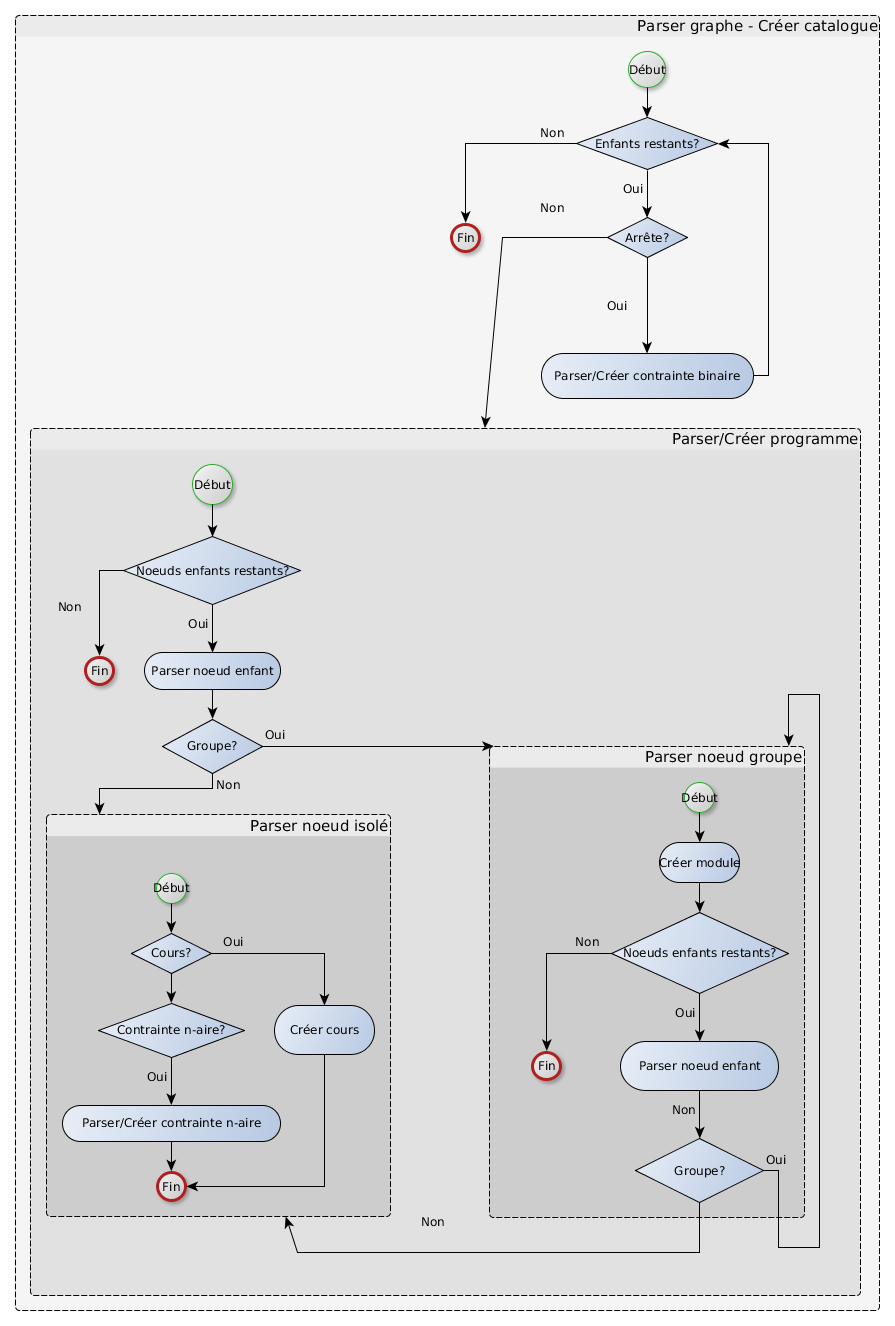
\includegraphics[width=\textwidth]{graphml_parser}
\end{figure}

%  Comme expliqué dans l'introduction de cette section, chaque élément peut avoir un enfant, est identifié par un tag, peut avoir des attributs et contient de l'information. 

%  la structure plus détaillée d'un nœud est la suivante:

% \begin{lstlisting}
% <node id="parentID::nodeID" [GROUP]>
%   <(...)>
%   </(...)
%   <NodeLabel>
%     NAME
%   </(...)
%   <(...)>
%   </(...)>
% </node>
% <graph id="parentID">
%   <node id (...)>
%   <node id (...)>
% </graph>
% \end{lstlisting}

% Il y a donc quatre informations à extraire;
% \begin{enumerate}
%   \item l'identifiant du nœud parent (parentID);
%   \item l'identifiant du nœud (nodeID);
%   \item son nom (NAME);
%   \item est-ce un groupe? (GROUP)
% \end{enumerate}

% La structure de graphe imposée à la commission est la suivante; 

% \begin{itemize}
% \item les modules et programmes sont représentés par des nœuds \textit{Group};
% \item les cours sont représentés par des simple nœuds;
% \item les dépendances par des arrêtes.
% \end{itemize}

% Notez que chaque cour et module \textbf{DOIT} se trouver dans un programme. En effet, \textit{nœuds groupes} sans parents sont interprétés comme programmes. Cela nous permet de distinguer les modules des programmes, sans devoir ajouter une convention de couleur sur les boites pour les différencier.  

% L'algorithme de parsing est donc relativement simple.

% On a;
% \begin{itemize}
%   \item une méthode qui parse les arrêtes; 
%   \item une méthode qui parse les nœuds;
%   \item une méthode qui aprse les programmes et ses enfants;
%   \item une méthode qui parse les modules et ses enfants;
%   \item une méthode qui parse les cours.
% \end{itemize}

% On crée au préalable un \textbf{objet} catalogue. Chacune des méthodes listées précédemment renvoie un \textbf{objet} Cours, Module, Programme, Contrainte. Ces objets sont ajoutés au catalogue en respectant leur hiérarchie. Un cours aura donc comme parent un module ou un programme. 


% \begin{lstlisting}
% FOREACH element in graph do
% - IF node -> 
%   parse node
%   - IF program -> 
%     parse program (extract informations and add to catalog)
%     (1) parse childs
%       - IF module
%         -> parse module (extract informations and add to parent)
%         -> parse childs (go_to (1))
%       - IF course
%         -> parse course (extract informations and add to parent)


% - IF edge -> 
%   parse edge
%     retrieve sources
%     retrieve destinatinations
%     retrieve constraint type
%     FOREACH course in destinations do
%       add new contraint to course
% \end{lstlisting}


Une fois le parsing terminé, toutes les informations contenues dans chacun des \textbf{objets} cours, modules et programmes et contraintes sont ajoutées dans la table correspondante en base de donnée. 


\subsection{Gestion des contraintes}
\label{constraint_mgmt}
Les contraintes sont vérifiées au niveau du modèle \textit{StudentProgram}, le modèle qui contient les informations à propos des programmes de cours des étudiants (C'est ce modèle qui appelle le module \textit{ConstraintsChecker}). 

Le module \textit{ConstraintsChecker} est divisé en deux parties. D'un coté nous avons les contraintes. Tout les types de contraintes héritent de la super classe \textit{Contrainte} qui, en plus de constructeur ne contient qu'une seule méthode \textbf{Check}. De l'autre coté, nous avons les entités qui représentent les modèles \textit{Course}, \textit{Module} et \textit{Program}

Les grand principes du vérificateur de contraintes sont illustrés sur le diagramme \ref{fig:constraint_checker_diagram} à savoir;

\begin{figure}
\centering
\caption{Vérification des contraintes}
\label{fig:constraint_checker_diagram}
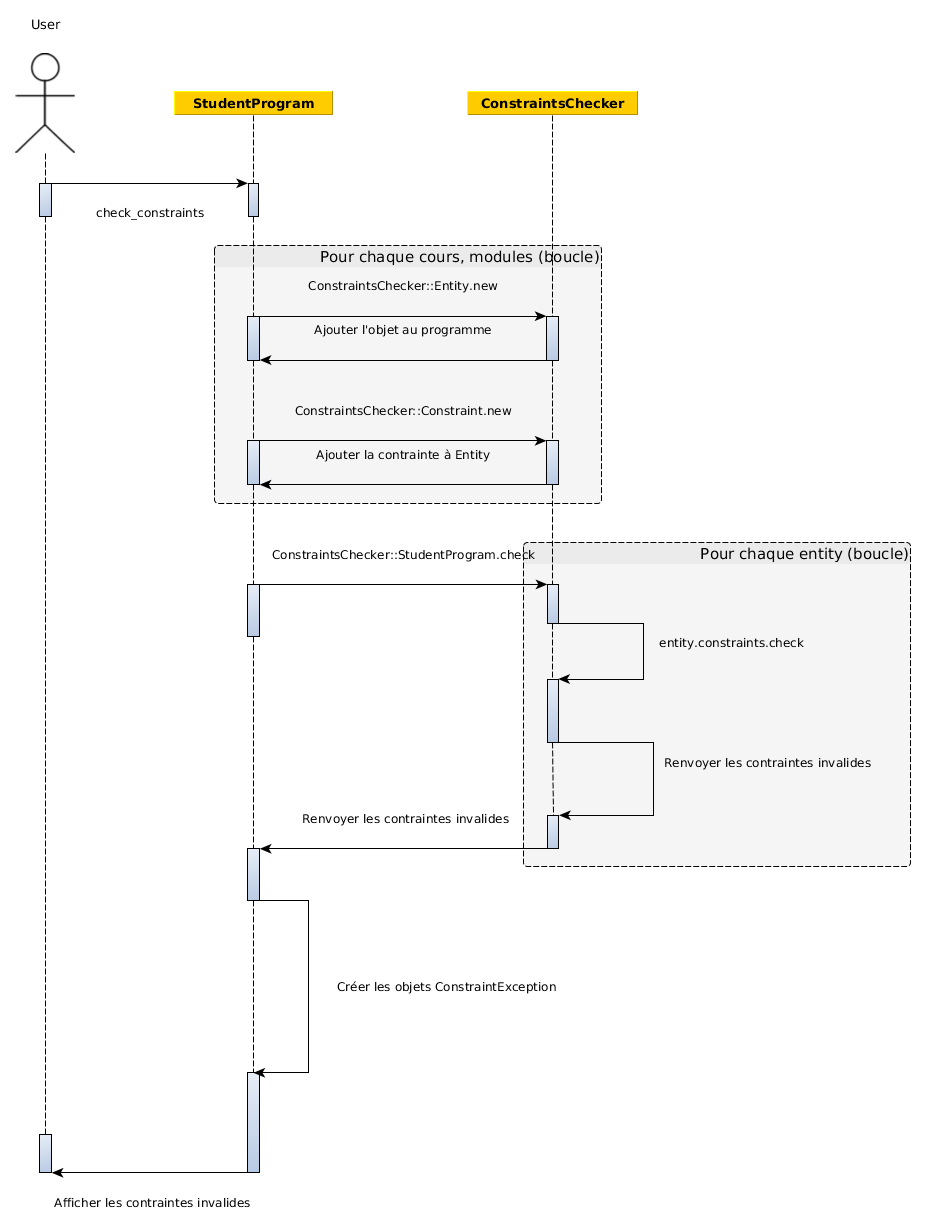
\includegraphics[width = \textwidth]{constraints_checker_diagram}
\end{figure}

\begin{enumerate}
\item lorsque l'étudiant veut vérifier les contraintes de son programme la méthode \textit{check\_constraints} est appelée; cette méthode crée, pour chacun des éléments qui constitue son programme (cours, modules) un objet \textit{ConstraintChecker.Entity}  qui va contenir toutes les informations nécessaire à la vérification des contraintes; la structure qui contient tout ces objets et un arbre, dont la racine est l'objet \textit{ConstraintsChecker.Entity\:\:StudentProgram}
\item chaque modèle de la base de donnée (\textit{Course, PModule}) contient une méthode \textit{get\_(...)\_object)} qui va créer l'objet \textit{Entity} correspondant;
\item cette méthode, s'occupe aussi d'ajouter à l'objet \textit{Entity} les contraintes qui le caractérisent;
\item une fois tout les objets créés, la méthode \textit{check} de l'objet\\ 
\textit{ConstraintChecker.Entity.StudentProgram} est appelée; cette méthode appelle la méthode \textit{check} de chacun de ses enfants et récupère les contraintes invalides;
\item une fois la vérification terminée, un objet \textit{ConstrainteException} est créé pour chaque contrainte non vérifiée; on pourra ainsi avoir accès aux informations de chacune de ces contraintes dans la vue à laquelle l'étudiant à accès pour vérifier ses contraintes, et surtout attacher une justification à cette \textit{exception} pour négocier la valider du programme avec la commission de programme.
\end{enumerate}



% \subsubsection{Entités}
% \textit{Entity} est la classe qui représente les objets traités par le module \textit{ConstraintsChecker}. Entity étends la classe OpenStruct. Openstruct est une librairie qui permet de créer des objets à la volée. Pour chaque paramètre passé à un objet \textit{OpenStruct} \cite{OpenStruct}, un attribut sera créé ainsi que les méthodes pour le modifier et y accéder. On évite ainsi de devoir modifier la classe \textit{Entity} et ses enfants {Course, PModule} lorsque l'on veut rajouter une contrainte ou une nouvelle propriété par exemple.

% Nos différents objets sont stockés sous forme d'arbre. La racine est l'objet \textit{ConstraintsChecker::Entities::StudentProgram}, et les enfants sont les différents objets \textit{Course} et \textit{PModule}, tous étendant le super-type \textit{Entity}.

% Un objet \textit{entity} contient essentiellement;

% \begin{itemize}
%   \item un attribut \textbf{constraints} qui contienne les différentes contraintes de l'objet;
%   \item un attribut \textbf{childrens} qui contient les références vers ses enfant dans l'arbre;
%   \item un attribut \textbf{parent} qui contient la référence vers son parent dans l'arbre;
%   \item une méthode \textbf{find\_children(children\_id, children\_type)} qui permet d'effectuer une recherche sur ses enfants. Le paramètre \textit{children\_type} permets de spécifier le type d'enfant que nous recherchons (Cours, PModule);
%   \item une méthode \textbf{search(children\_id, children\_type)} qui permet d'effectuer une recherche dans tout l'arbre. Cette méthode est utilisé dans les methodes \textit{check} des différentes contraintes pour retrouver des objets \textit{Course}. (Retrouver une dépendance par exemple). L'algorithme est le suivant;
%   \begin{lstlisting}
%   - Retrouver la racine de l'arbre
%   - Appeler find_children sur ses enfants
%   \end{lstlisting}
%   \item une méthode \textbf{check} qui vérifie ses contraintes et celle de ses enfants;
%   \item des méthodes relatives aux différentes contraintes, comme \textit{count\_credits}, \textit{check\_max}, \textit{check\_min}, \ldots
% \end{itemize}

% Ces objets sont construits dans les différents modèles de l'application. L'idée, dans chacun de ces modèles (Course, PModule, Constraint) est d'avoir une méthode get\_[model\_name]object qui va créer l'objet correspondant.

% Dans le cas du modèle \textit{Course}, la méthode est la suivante:


% \textbf{Course}

% \begin{lstlisting}
% def get_course_object(start_year, end_year)
%   course = ConstraintsChecker::Entities::Course.new(name: self.name, id: self.id, start_year: start_year, end_year: end_year, parent_id: self.p_module_id, credits: self.credits, mandatory: self.mandatory?)
%   self.constraints.each do |c|
%     course.add_constraint(c.get_constraint_object(course))
%   end
%   return course
% end
% \end{lstlisting}


% Les paramètre \textit{start\_year} et \textit{end\_year} identifient l'année académique au cours de laquelle un cours a été suivie dans un programme d'étudiant. Ces informations sont utilisés lors de la vérification des dépendances. 

% Dans le cas d'un prérequis  par exemple, l'algorithme va vérifier que l'année académique durant laquelle a été suivie le cours est strictement antérieure à l'année académique du cours pour le quel il est un prérequis. Ce mécanisme gère aussi bien les années réussies que les années ratées. En effet, dans le cas d'une année raté, la commission aura au préalable sélectionner les cours qui on été réussis. Les cours ratés (qui ne sont pas sélectionnés) seront retiré de l'année en question. Il ne seront donc pas présent dans \textbf{objet} StudentProgram lors de la vérification des contraintes. 

% Comme expliqué plus haut, on peut passer au constructeur de \textit{Course} tout ce que l'on veut, grâce à OpenStruct \cite{OpenStruct}.

% Rien ne nous oblige à passer par le modèle \textit{Constraint} pour ajouter les contraintes. Comme expliqué dans la section \ref{rails_arch} (présentant l'architecture de l'application) , seul les dépendances sont représentés par l'objet \textit{Constraint} en base de données. En effet la plupart des données relatives à ces contraintes sont, en plus d'être présentes en base de données, assez volatiles, car elles peuvent être modifiées régulièrement via l'import de fichiers excels. Nous évitons ainsi de surcharger notre architecture avec des objets dont l'utilité est plus que relative. Pour revenir à ce type de contraintes, il est préférable de les ajouter dans la méthode \textit{get\_[model\_name]object} (la méthode du modèle qui crée l'objet \textit{Entity}.

% \textbf{PModule}

% \begin{lstlisting}
%   def get_p_module_object(mandatory)
%     p_module = ConstraintsChecker::Entities::PModule.new(id: self.id, name: self.name)
%     p_module.add_constraint(ConstraintsChecker::Constraints::Min.new(p_module, self.min))
%     p_module.add_constraint(ConstraintsChecker::Constraints::Max.new(p_module, self.max))
%     self.sub_modules.each do |m|
%       p_module.add_children(m.get_p_module_object(true))
%     end

%     if mandatory
%       course_ids = []
%       self.courses.each do |course|
%         course_ids << course.id
%       end
%       p_module.add_constraint(ConstraintsChecker::Constraints::Mandatory.new(p_module, course_ids))
%     end
%     return p_module
%   end
% \end{lstlisting}

% Le paramètre \textit{mandatory} sert à identifier si le module est obligatoire ou non. Cela est utile pour vérifier si les cours d'un module obligatoire on bien été suivis.
% Nous avons ici un exemple de contraintes (Min \& Max) qui ne sont pas ajoutées en passant par le modèle \textit{Constraint}. 


% \subsubsection{Contraintes}
% L'idée, pour chaque type de contraintes, est d'étendre la super-classe \textit{Constraint} en ré-implémentant la méthode \textit{check} pour qu'elle corresponde au comportement recherché. Cette méthode renvoie un \textit{hash}, spécifique à chaque type de contraintes, contenant les résultats de la vérification.

% Par exemple, pour les dépendances entre les cours nous avons deux types. Les dépendances binaires, qui correspondent à un prérequis ou corequis entre deux cours, et les dépendances n-aire qui correspondent à un ensemble de prérequis ou corequis entre plusieurs cours avec une condition sur cet ensemble de contraintes. Cet ensemble peut être une disjonction (OR) de contraintes par exemple, exprimant qu'il faut choisir au moins une des dépendances, ou une disjonction exclusive (XOR), exprimant qu'il faut choisir une et une seule dépendance. 

% Prenons l'exemple des dépendances binaires. Nous avons une classe \textit{BinaryConstraint} qui ne ré-implémente pas la méthode check de sa super-classe \textit{Constraint} car elle sert de super-classe pour les deux classes représentant les deux types de contraintes; \textit{Prerequisite} et \textit{Corequisite}. 

% \begin{description}
%   \item[Corequisite] La méthode check va appeler la méthode \textit{find\_course} du cours en question, qui va remonter jusqu'à la racine (le StudentProgram), et chercher si le corequis du cours est présent dans le programme de l'étudiant.  S'il est présent, il va vérifier qu'il n'est pas suivit dans une année postérieure au cours pour le quel il est un corequis (conformément à la définition d'un prérequis \ref{contraintes}). Si la vérification précédente échoue, ou si le cours n'est tout simplement pas présent, le message ``corequisite\_missing :[course\_id]'' est envoyé.
%   \item[Prerequisite] La méthode check se comporte comme celle de \textit{Corequisite}, à la différence que la vérification de l'année académique est plus stricte: le cours doit être suivit dans une année strictement antérieure (conformément à la définition d'un prérequis \ref{contraintes}). 
% \end{description}

% Dans le cas d'un ensemble n-aire de contraintes, il y a essentiellement deux points qui diffèrent;
% \begin{enumerate}
%   \item l'existence d'une méthode \textit{find\_dependancies} qui récupère les \textit{course\_id} manquants pour la contrainte en question en vérifiant aussi les années académiques;
%   \item une vérification sur la taille de la liste, correspondant à la condition qui régit cet ensemble de contrainte. Dans le cas d'un ensemble disjonctif (OR), il faut vérifier que le nombre de \textit{course\_id} renvoyé soit strictement inférieure au nombre de dépendances du cours, pour vérifier qu'il y ai au moins une dépendance qui est choisie, conformément à la logique d'une disjonction. Dans le cas d'un ensemble disjonctif exclusif (XOR), il faut vérifier qu'il n'y aie qu'une et une seule dépendance choisie, conformément à la logique d'une disjonction exclusive.
% \end{enumerate}

% Pour vérifier ces contraintes, l'objet \textit{Catalog} appelle sur chacune des contraintes de ses enfants et de leur enfants leur méthode \textit{check}, puis renvoie les contraintes qui ne sont pas respectée. Après, l'objet du modèle \textit{StudentProgram} correpondant récupère ces contraintes non respectées et crée les objets \textit{ConstraintException}.

\subsubsection{Ajout d'un nouveau type de contraintes}

Pour ajouter un nouveau type de contraintes, il faut procéder comme suit:

\begin{enumerate}
  \item si le type de la contrainte ne rentre pas dans la catégorisation des contraintes déjà existantes (BinaryConstraint, PropertyConstraint, NaryConstraint), il faut créer une nouvelle classe. Sinon, il suffit d'étendre la classe existante;
  \item implémenter la méthode \textit{check} de cette contrainte avec le comportement désiré;
  \item dans la méthode \textit{get\_object} du modèle concerné par la contrainte, créer et ajouter l'objet contrainte et ajouter les informations nécessaires dans l'objet créé par le modèle; par exemple, si je rajoute une contrainte sur les crédits, il faut passer le paramètre \textit{credits: value} au constructeur de l'objet \textit{Entity::Course}.
\end{enumerate}



\subsection{Importation du formulaire Excel}
Le module est composé de deux parties: 
\begin{enumerate}
\item un \textit{Reader} qui propose une fonction pour récupérer sous forme de tableau de \textit{Hash} les informations d'une page Excel, en lui fournissant \textbf{le nom de la page}, ainsi que \textbf{la propriété qui est utilisée pour identifier l'objet} (Le sigle pour les cours par exemple);
\item un \textit{Writter} qui propose une fonction pour écrire des données dans une page d'un document Excel.
\end{enumerate}

L'intérêt de fournir une abstraction supplémentaire se situe sur la structure des documents échangés avec l'utilisateur. En effet, chaque document comporte plusieurs pages. Chacune d'entre elles contient des informations sur un des objets (Course, Sub-Module, Modules ou Program). Ces informations sont représentées par le Modèle \textit{Property} en base de données. Il est donc nécessaire d'avoir la première ligne de chacune de ces pages réservée pour y mettre le header afin de savoir pour chaque ligne à quel type de propriétés l'information appartient.

Pour les cours par exemple, ce header est de la forme:
\begin{table}[H]
\centering
\begin{tabular}{| c | c | c | c |}
\hline
\textbf{Sigle} & \textbf{Crédits} & \textbf{...} & \textbf{...}\\
\hline
\end{tabular}  
\end{table}

Ici, il n'a pas été nécessaire d'utiliser une abstraction \textit{Entity}, contrairement aux autres modules (GraphParser, ConstraintsChecker), pour représenter les données. En effet, nous ne manipulons que des tableaux de données, et surtout nous n'avons pas à nous occuper des inclusions entre les différents objets, ce module traitant exclusivement leur propriétés. C'est pourquoi ce module et l'application s'échangent des \textit{Hash}. 


Le \textit{Writter} est appelé lorsque l'utilisateur télécharge un template de formulaire Excel après avoir créé le catalogue. 

Le \textit{Reader} est appelé à chaque fois que l'utilisateur met à jour les données d'un catalogue de cours via le formulaire Excel. 


Notez que ce fichier est stocké, tout comme celui contenant le graphe, sur le cloud \textit{Amazon}.
\section{Qualité}
Dans cette section, il sera question de la qualité du code qui a été produit pour développer l'application. 

\subsection{Maintenabilité}

Tout au long du développement, les bonnes pratique de \textit{Ruby on rails} on été suivis à la lettre à savoir:
\begin{itemize}
\item éviter d'avoir de la logique dans les vues et les alléger au plus possible;
\item alléger au plus possible les contrôleurs;
\item déléguer au plus possible le travail au modèles.
\end{itemize}

Cependant, avec cette pratique, on se retrouve très vite avec de larges modèles. Avoir des larges classes est un comportement que l'on veut éviter, afin de renforcer la cohésion de celles-ci et diminuer leur couplage. C'est pourquoi certaines fonctionnalités on été implémentées dans des modules externes (ConstraintsChecker, GraphParser, XlsParser).

À l'avenir, si l'on souhaite changer la façon dont on importe la structure d'un catalogue de cours par exemple, il suffira juste de changer l'appel au module (méthode \textit{import\_graph}) dans le modèle \textit{Catalog}. Plus simplement, si l'on souhaite importer des informations supplémentaires lorsque l'on importe ce graphe, il suffit de se rendre dans le module correspondant et non partir à la recherche du bout de code dans un modèle dont la taille se chiffrerait en milliers de lignes de code.

Au niveau de l'optimisation, la gem \textit{bullet} a été utilisée pour détecter et corriger les endroits ou apparaissaient des \textit{N+1 queries}. 

Les \textit{N+1 queries} sont un ensemble de requêtes qui pourraient être réduites à une seule. Les accès à la base de données étant couteuses en ressources, il est primordial de les réduire au minimum afin de garantir une expérience fluide lors de l'utilisation de l'application. 

Lorsque l'on récupère un module et ses cours par exemple, il est considérablement plus rapide de récupérer toute les données à l'aide d'une requête (à l'aide de la méthode \textit{includes}, plutôt que de récupérer le module, puis d'itérer sur celui-ci et de récupérer les cours un à un. 


\subsection{Tests}
La plupart des test bas niveaux ont été réalisés dans les modules (\textit{ConstraintsChecher}, \textit{XlsParser}, \textit{GraphParser}) à l'aide de RSpec. RSPec est un outil de testing orienté \textit{Behaviour-Driven Development}. Il a été utilisé en définissant les exigences d'une fonctionnalité, avant de commencer le développement de celle-ci.

Pour les test hauts niveaux des fonctionnalités, des scénarios on été créés et testés en temps réel. Chacun de ces scénarios, ainsi que leur résultat est décrit dans le chapitre Validation \ref{validation}
\section{Conclusion}

Ce chapitre clos l'explication et la description des fonctionnalités de la solution. Le chapitre qui suit analysera la qualité des fonctionnalités de l'application, à l'aide de scénarios, afin d'identifier ses limites et de pouvoir proposer, dans le dernier chapitre, des pistes de travaux futurs pour la solution. 
